% kapitel2.tex
\chapter{Implemented Changes}
\label{chapter:implementedChanges}

This work extends Tour4Me, which is an application written in C++ and HTML. 
The implemented interface uses C\# as its programming language to enable easy porting of the webapplication to a desktop or mobile application.
To improve the query times, a spatial database was added. 
Reasons for and positive effects of this decision are described in the following section.

Furthermore, not only the language and data access was changed.
New options and parameters to improve the customizability of preferences for a generated tour were added as well.
These changes had to be incorporated into an upgraded frontend design (see sections \ref{subsec:interfaceAndFrontendChanges} and \ref{sec:parameterChanges}) as well as into the backend and all solvers (see section \ref{sec:algorithmicChanges}). 


\section{Application}
\label{sec:application}

\subsection{New Architecture}
\label{sec:newArchitecture}

For the new application, the architecture had to be re-structured.
An illustration of the new design is shown in figure \ref{fig:architecture}.
Instead of reading the data for the graph from a static .txt file, which contains all the nodes and edges for Dortmund, a database is used to manage the nodes, edges, their additional information and the relationships between them. 
It can be filled with the data needed by using an import python script that creates an osmnx-graoh \#TODO add all references for a user specified location. 
From this graph, the nodes and edges can be extracted alongside their additional information.
For the current use case, nodes are stored with their ID, which is transformed into a uuid, their latitude and longitude coordinates as well as their elevation profile and tags of the surroundings they are placed in.
The elevation data has to be accquired from a different source than osm, since they do not use a height profile. 
A few open source providers were available, but ultimately, Open-Elevation\footnote{\url{https://open-elevation.com/}, last accessed: \today} was used. 

Since most open source providers have a limited bandwidth to supply users with data based on their api-calls, the opportunity to use a locally hosted version that Open-Elevation offered was very important to assure usability.
When using the python script to create and fill the database and its tables, the Open-Elevation data needs to be available.
A local docker container with the respective data can be used to access the needed information without being bound to the servers and their throughput boundaries.

The used database is Microsoft SQL Server Management Studio, because it can handle spatial data, supports spatial queries and works well in combination with the C\# implementation.

The backend is written in C\#, as it allows for the opportunity to also create a mobile- or desktop application in addtion to the web application that already exists (see \ref{sec:futureWork}).
Furthermore, it allows for using SQL queries and filtering using the LINQ ??? \# TODO find doku etc.

The frontend is implemented using HTML, CSS, JavaScript and C\# code behind. 
Here, the base-styling is done using bootstrap, but additional custom CSS is added to create a nature-based color palette (\#TODO references to color therory stuff?) as well as several effects for the side and bottom menus.
To realise the communication between frontend and backend, ajax queries are used.

The map is a leaflet visualization that shows Open Street Map data.
It allows to set markers, add a search bar, create polygons - which are used to illustrate the generated routes - and offers an open source map view. 




\begin{figure}[H]
	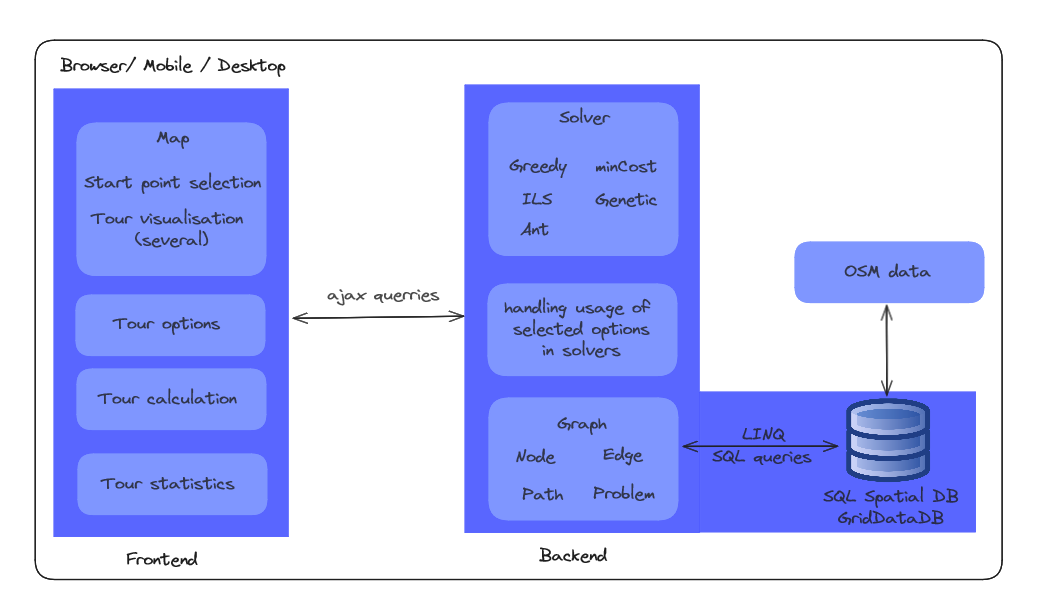
\includegraphics[width=0.9\linewidth]{bilder/Implementation Architecture.png}
	\caption{Visualization of the used architecture}
	\label{fig:architecture}
\end{figure}

\subsection{Database}
\label{subsection:database}

\subsection{Interface and Frontend changes}
\label{subsec:interfaceAndFrontendChanges}

\begin{figure}[H]
	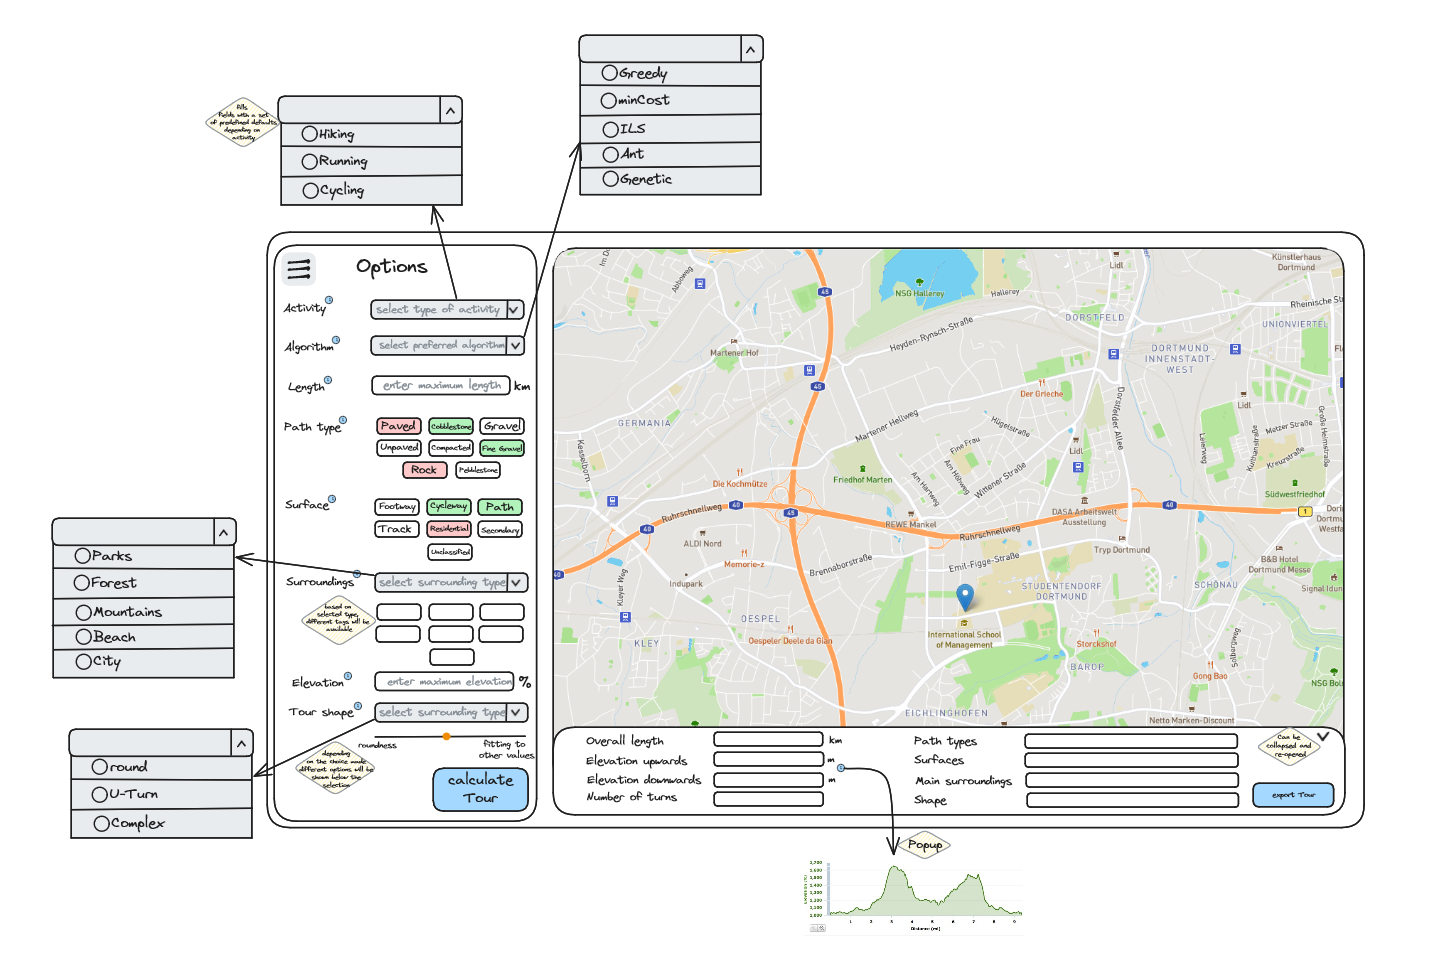
\includegraphics[width=0.9\linewidth]{bilder/Concept new Frontend design.png}
	\caption{Design concept for the frontend view, including descriptions for drop-downs and pop-ups}
	\label{fig:frontendConcept}
\end{figure}


\begin{figure}[H]
	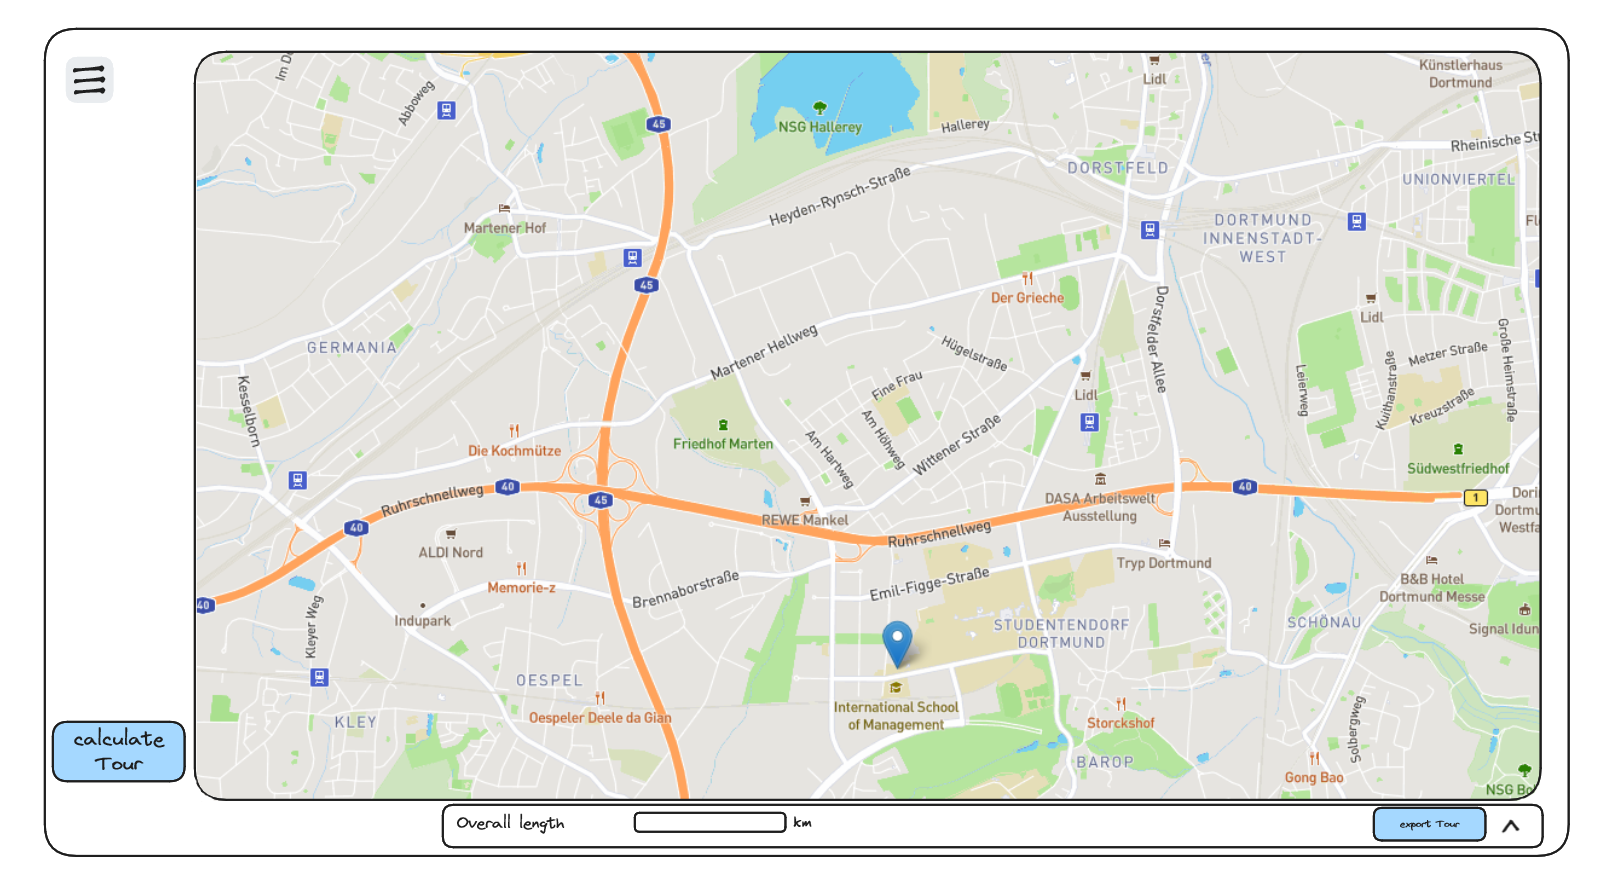
\includegraphics[width=0.9\linewidth]{bilder/Concept burger menu and stats hidden.png}
	\caption{Design concept for the frontend view with all menus folded}
	\label{fig:frontendConceptMenusClosed}
\end{figure}


\begin{figure}[H]
	\begin{subfigure}[t]{0.49\linewidth}
		\centering
		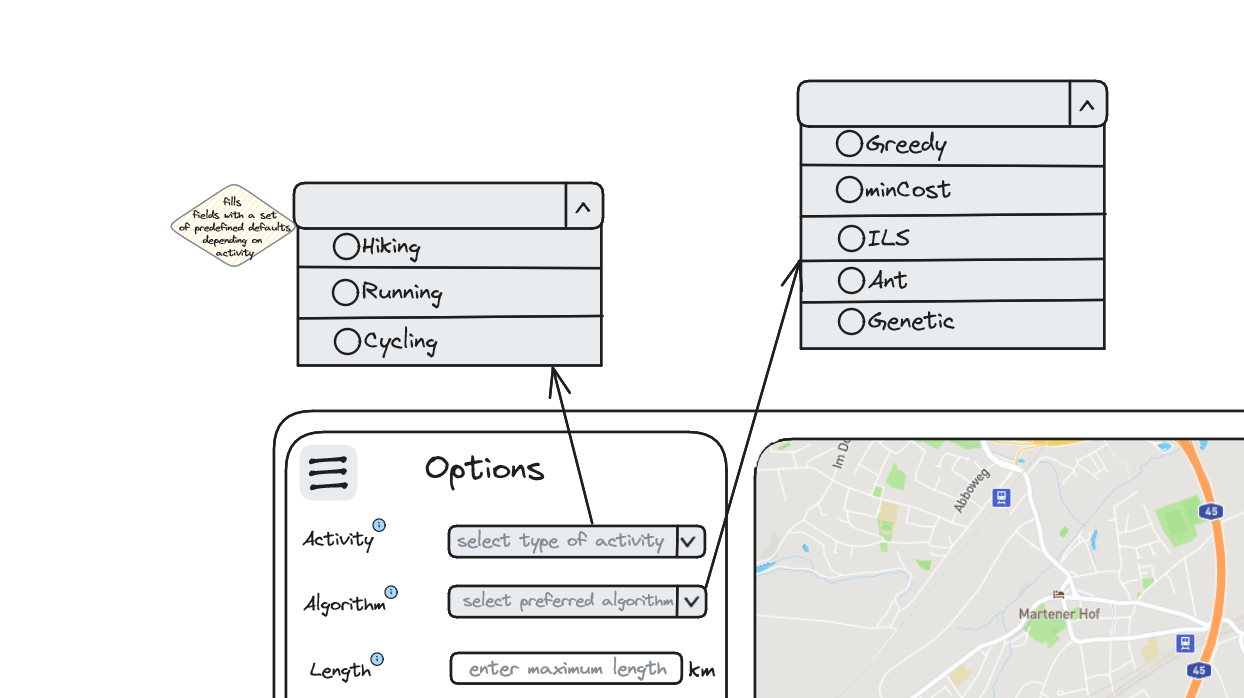
\includegraphics[width=\linewidth]{bilder/Concept closeup activity, algorithm.png}
		\caption{Design concept for the frontend view, closeup of activity and algorithm dropdowns}
		\label{fig:frontendConceptCloseupDropdowns}	
	\end{subfigure}
	\hfill
	\begin{subfigure}[t]{0.49\linewidth}
		\centering
		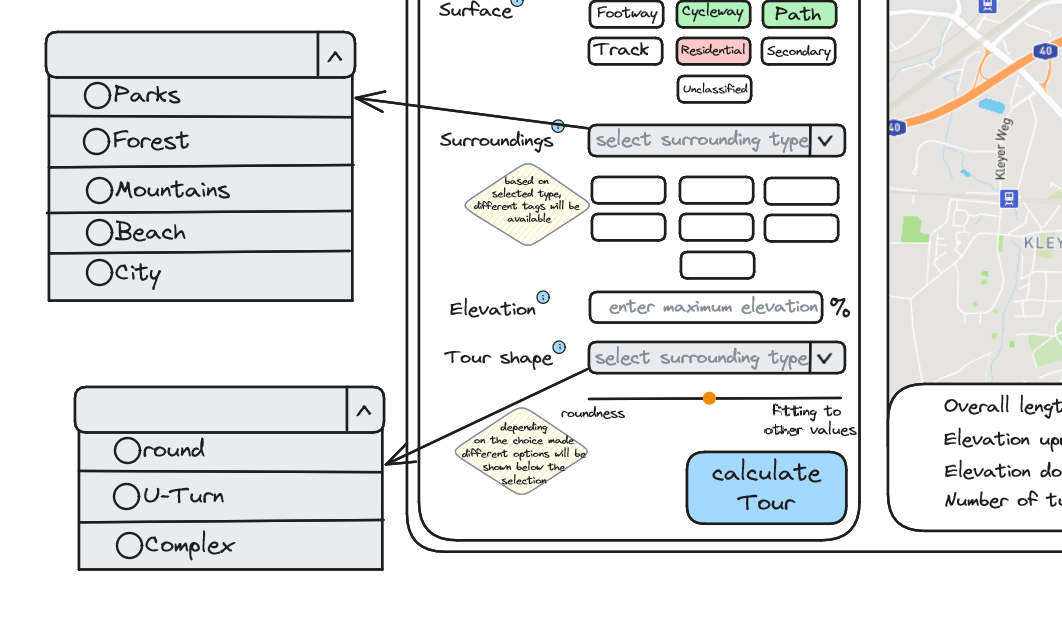
\includegraphics[width=\linewidth]{bilder/Concept closeup surroundings, tour shape.png}
		\caption{Design concept for the frontend view, closeup of a surrounding and Tour shape}
		\label{fig:frontendConceptCloseupButtons}		
	\end{subfigure}
\end{figure}


\begin{figure}[H]
	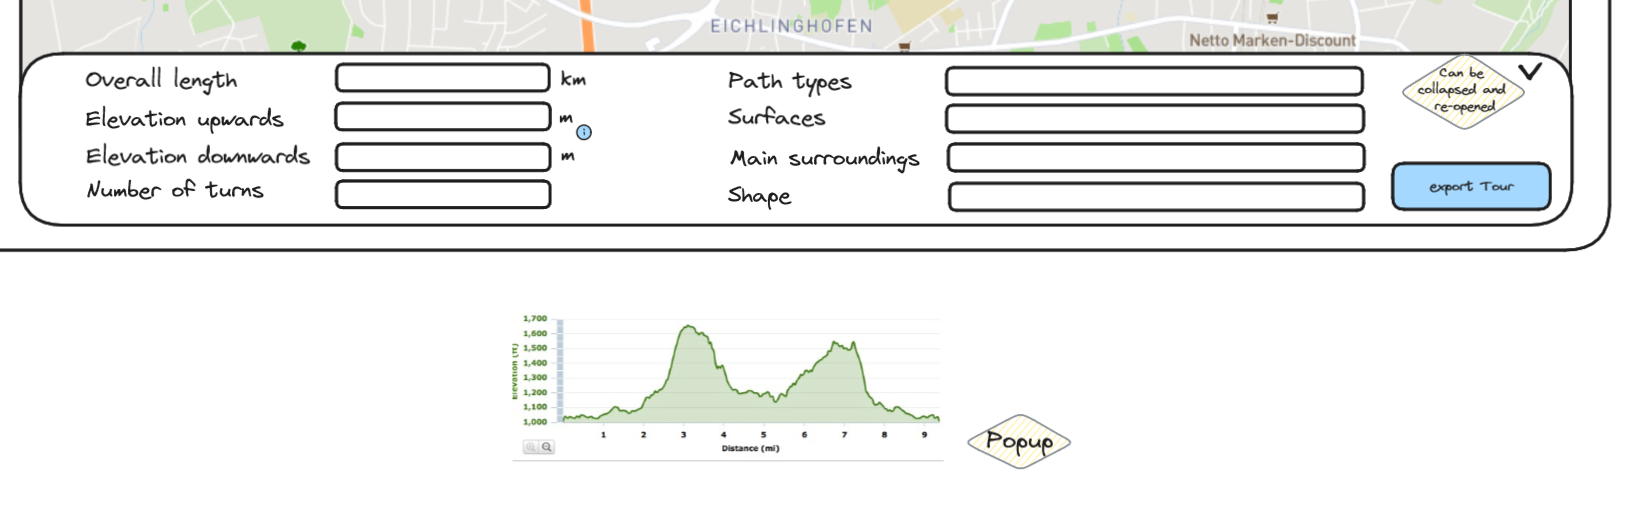
\includegraphics[width=0.9\linewidth]{bilder/Concept closeup tour stats, elevation profile.png}
	\caption{Design concept for the frontend view, closeup of the results view}
	\label{fig:frontendConceptResultsCloseup}
\end{figure}



\section{Algorithmic changes}
\label{sec:algorithmicChanges}

\subsection{Ant Colony}
\label{subsec:antColonyImplementation}

\subsection{Genetic Algorithms}
\label{subsec:geneticAlgorithmsImplementation}

\subsection{Simulated Annealing}
\label{subsec:simulatedAnnealingImplementation}

\section{Parameter changes}
\label{sec:parameterChanges}

